\documentclass[12pt,a4paper]{article}
%\usepackage{ctex}
\usepackage{amsmath,amscd,amsbsy,amssymb,latexsym,url,bm,amsthm}
\usepackage{epsfig,graphicx,subfigure}
\usepackage{enumitem,balance}
\usepackage{wrapfig}
\usepackage{mathrsfs,euscript}
\usepackage[x11names,svgnames,dvipsnames]{xcolor}
\usepackage{hyperref}
\usepackage[vlined,ruled,commentsnumbered,linesnumbered]{algorithm2e}
\usepackage{listings}
\usepackage{multicol}

\usepackage{tikz}
\usepackage{verbatim}
%\usepackage[active,tightpage]{preview}
\usepackage{preview}
\PreviewEnvironment{tikzpicture}
\usetikzlibrary{trees}


\renewcommand{\listalgorithmcfname}{List of Algorithms}
\renewcommand{\algorithmcfname}{Alg}

\newtheorem{theorem}{Theorem}
\newtheorem{lemma}[theorem]{Lemma}
\newtheorem{proposition}[theorem]{Proposition}
\newtheorem{corollary}[theorem]{Corollary}
\newtheorem{exercise}{Exercise}
\newtheorem*{solution}{Solution}
\newtheorem{definition}{Definition}
\theoremstyle{definition}


%\numberwithin{equation}{section}
%\numberwithin{figure}{section}

\renewcommand{\thefootnote}{\fnsymbol{footnote}}

\newcommand{\postscript}[2]
 {\setlength{\epsfxsize}{#2\hsize}
  \centerline{\epsfbox{#1}}}

\renewcommand{\baselinestretch}{1.0}

\setlength{\oddsidemargin}{-0.365in}
\setlength{\evensidemargin}{-0.365in}
\setlength{\topmargin}{-0.3in}
\setlength{\headheight}{0in}
\setlength{\headsep}{0in}
\setlength{\textheight}{10.1in}
\setlength{\textwidth}{7in}
\makeatletter \renewenvironment{proof}[1][Proof] {\par\pushQED{\qed}\normalfont\topsep6\p@\@plus6\p@\relax\trivlist\item[\hskip\labelsep\bfseries#1\@addpunct{.}]\ignorespaces}{\popQED\endtrivlist\@endpefalse} \makeatother
\makeatletter
\renewenvironment{solution}[1][Solution] {\par\pushQED{\qed}\normalfont\topsep6\p@\@plus6\p@\relax\trivlist\item[\hskip\labelsep\bfseries#1\@addpunct{.}]\ignorespaces}{\popQED\endtrivlist\@endpefalse} \makeatother


\definecolor{codegreen}{rgb}{0.44,0.68,0.28}
\definecolor{codegray}{rgb}{0.5,0.5,0.5}
\definecolor{codepurple}{rgb}{0.58,0,0.82}
\definecolor{backcolour}{rgb}{0.96,0.96,0.96}

\lstset{
language=C++,
frame=shadowbox,
keywordstyle = \color{blue}\bfseries,
commentstyle=\color{codegreen},
tabsize = 4,
backgroundcolor=\color{backcolour},
numbers=left,
numbersep=5pt,
breaklines=true,
emph = {int,float,double,char},emphstyle=\color{orange},
emph ={[2]const, typedef},emphstyle = {[2]\color{red}} }



\begin{document}
\noindent

%========================================================================
\noindent\framebox[\linewidth]{\shortstack[c]{
\Large{\textbf{Lab07-Trees}}\vspace{1mm}\\
VE281 - Data Structures and Algorithms, Xiaofeng Gao, TA: Qingmin Liu, Autumn 2019}}
%CS26019 - Algorithm Design and Analysis, Xiaofeng Gao, Autumn 2019}}
\begin{center}
\footnotesize{\color{red}$*$ Please upload your assignment to website. Contact webmaster for any questions.}

\footnotesize{\color{blue}$*$ Name: Sun Yiwen  \quad Student ID: 517370910213 \quad Email: sunyw99@sjtu.edu.cn}
\end{center}

{\color{blue}\textbf{Hint:} You can use the package \textbf{tikz} to draw trees.}

\begin{figure}[h]
\centering
\begin{tikzpicture}
	[thick,scale=0.8, every node/.style={scale=1.2}]
	\node {root}
	child {node {1}
		child {node {2}
			child {node {3}}
		}
		child [missing] {}
		child {node {3}
			child {node {2}}
		}
	}	
	child [missing] {}	
	child [missing] {}
	child [missing] {}	
	child [missing] {}	
	child { node {2}
		child {node {1}
			child {node {3}}
		}
		child [missing] {}
		child {node {3}
			child {node {1}}
		}
	}	
	child [missing] {}	
	child [missing] {}
	child [missing] {}	
	child [missing] {}	
	child { node {3}
		child {node {1}
			child {node {2}}
		}
		child [missing] {}
		child {node {2}
			child {node {1}}
		}
	};
	\end{tikzpicture}
	\end{figure}

\begin{enumerate}

\item	Red-black Tree
	\begin{enumerate}
		\item Suppose that we insert a sequence of keys 9, 3, 1 into an initially empty red-black tree. Draw the resulting red-black tree.
		
		\item Suppose that we further insert key 6 into the red-black tree you get in Problem (1-a). Draw the resulting red-black tree.
		
		\item Suppose that we further insert keys 2, 8 into the red-black tree you get in Problem (1-b). Draw the resulting red-black tree.
		
		\item Suppose that we further insert key 7 into the red-black tree you get in Problem (1-c). Draw the resulting red-black tree.
		
		\item Suppose that we further insert keys 4, 5 into the red-black tree you get in Problem (1-d). Draw the resulting red-black tree.
		
	\end{enumerate}
	
	When you draw the red-black tree, please indicate the color of each node in the tree.
For example, you can color each node or put a letter \textbf{b/r} near each node.

\begin{solution}
\quad\\
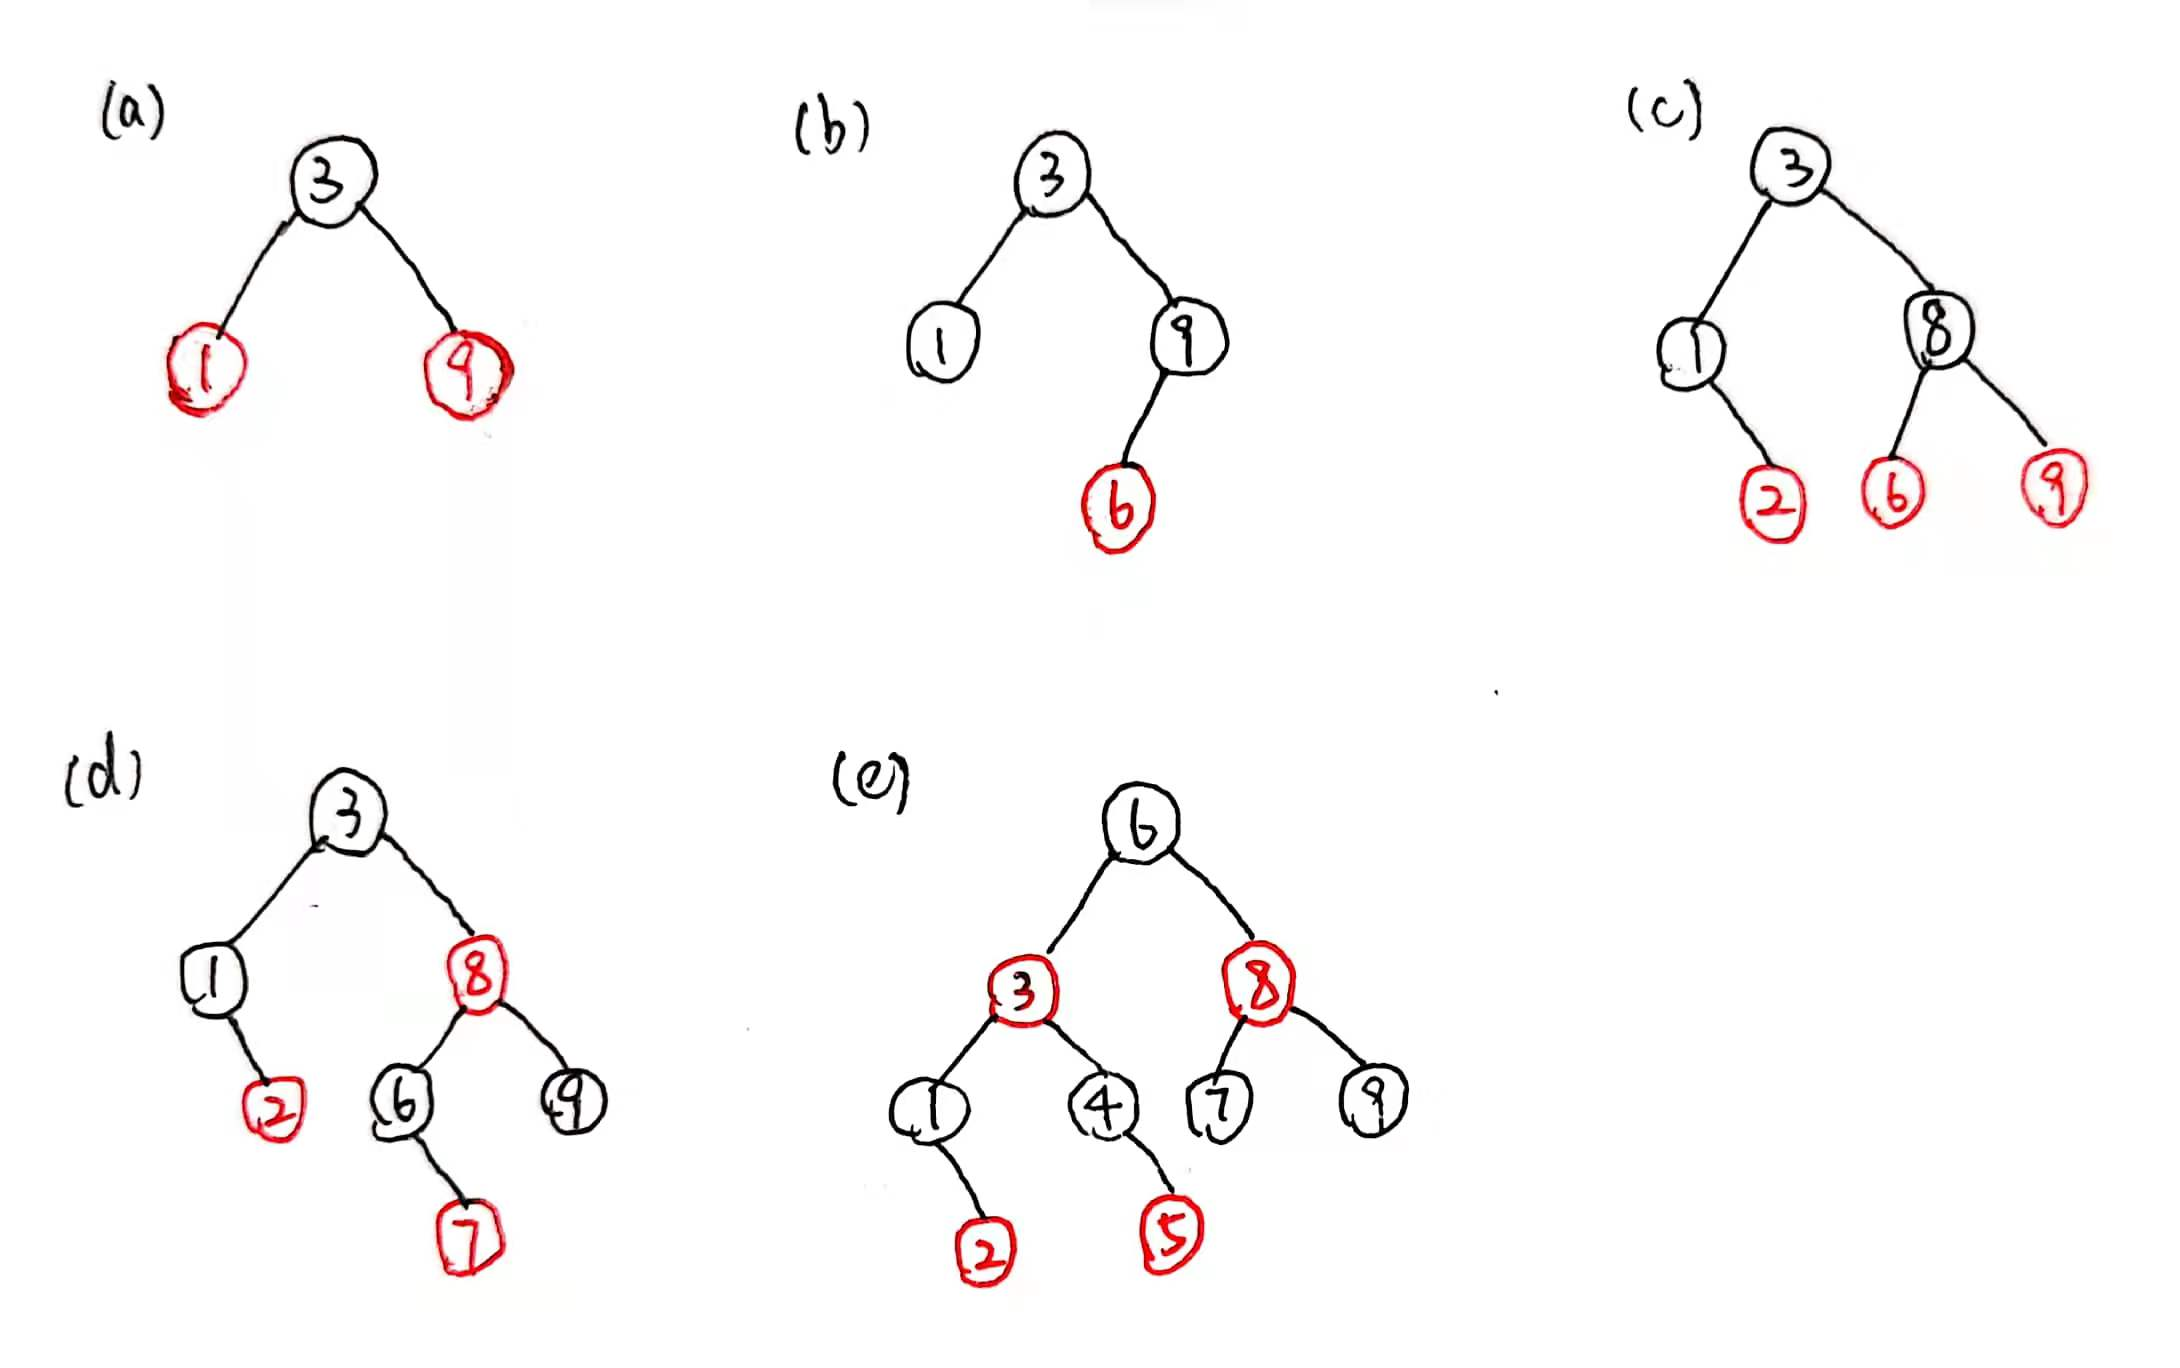
\includegraphics[scale=0.17]{p1.jpg}
\end{solution}

\item  Show the alphabet trie for the following collection of words: \{chicken, goose, deer, horse, antelope, anteater, goldfish, ant, goat, duck\}.

\begin{solution}
\quad\\
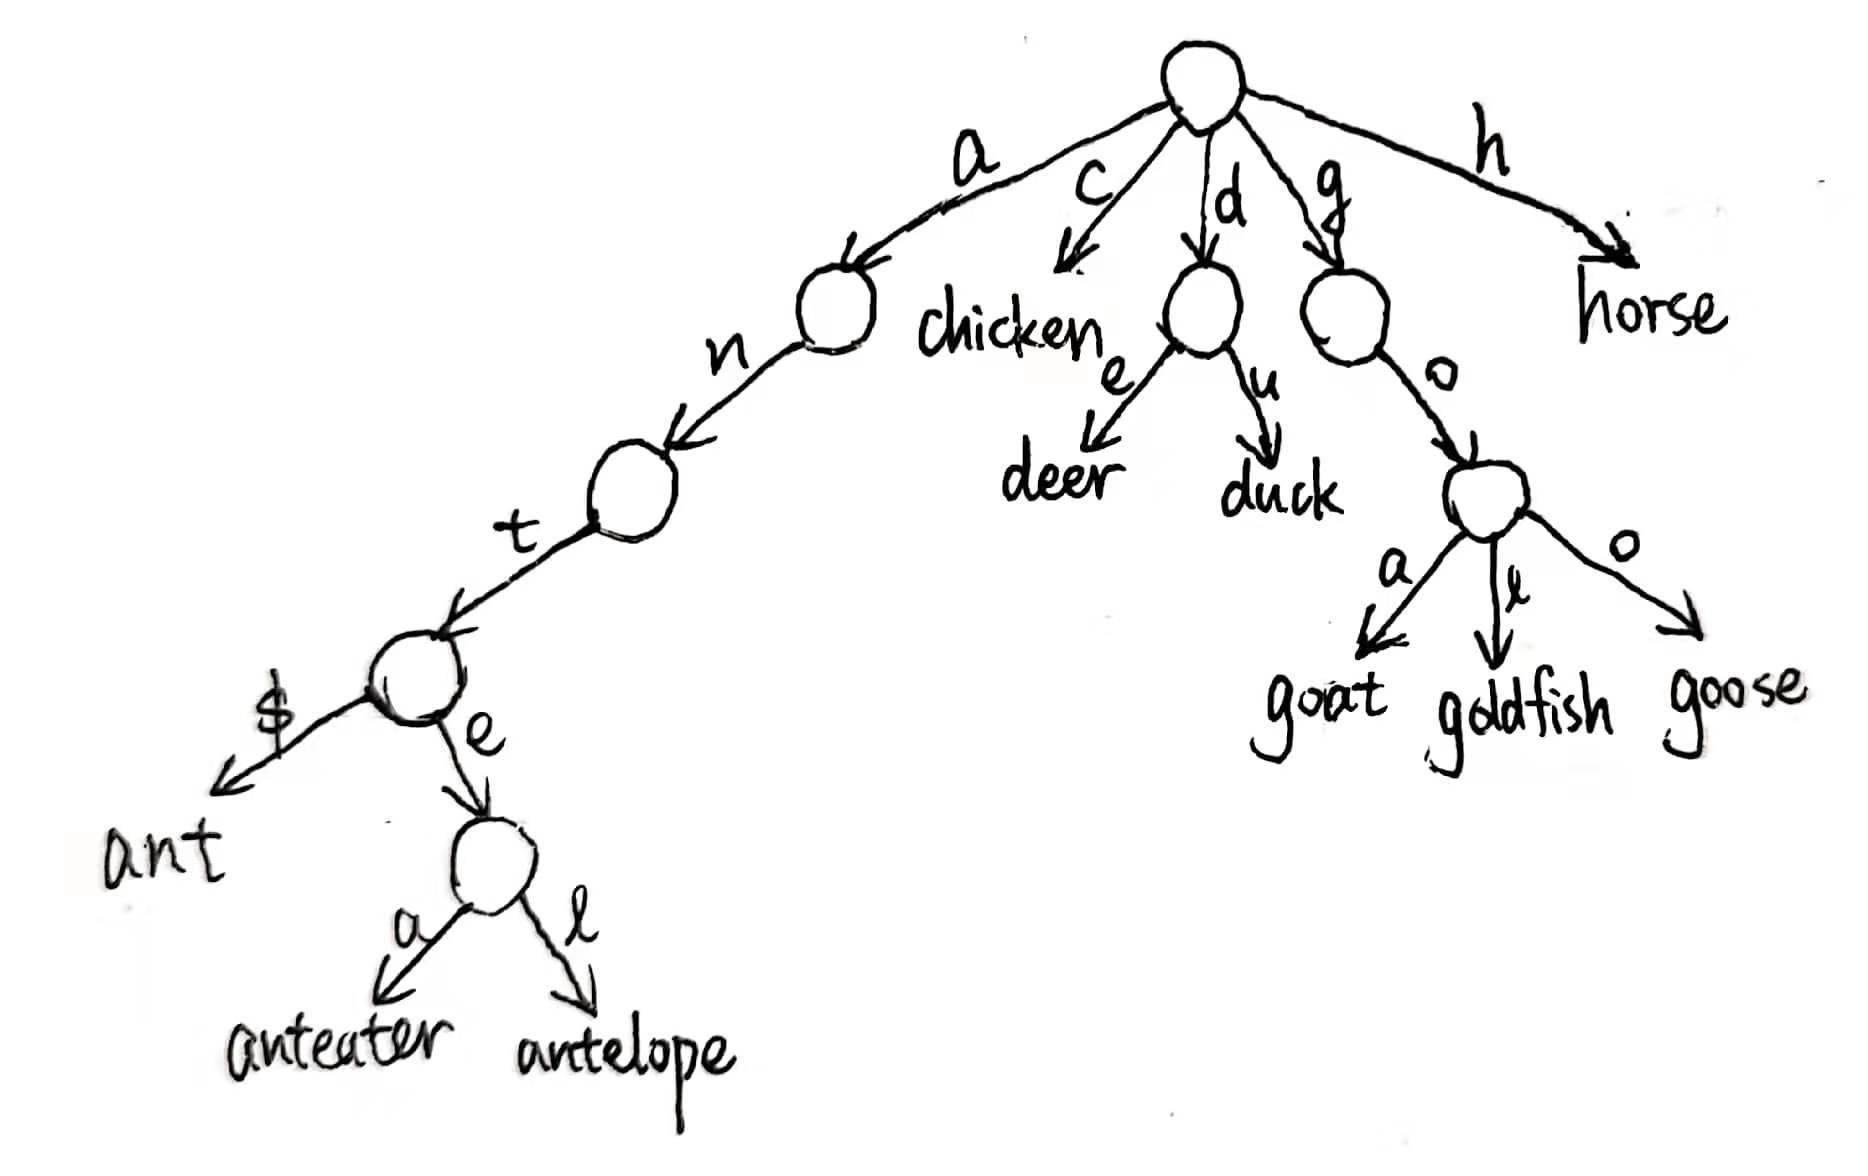
\includegraphics[scale=0.17]{p2.jpg}
\end{solution}

\item  Show that any arbitrary n-node binary search tree can be transformed into any other arbitrary n-node binary search tree using $O(n)$ rotations. 

	{\color{blue} Hint: First show that at most $n - 1$ right rotations suffice to transform the tree into a right-skewed binary
search tree.}

\begin{solution} 
\quad\\
As long as the tree is not transformed into a right-skewed tree (which is a right-going chain), repeatedly find some node y on the right spine that has a left child x and
then perform a right rotation on y, as shown in the following figure:\\
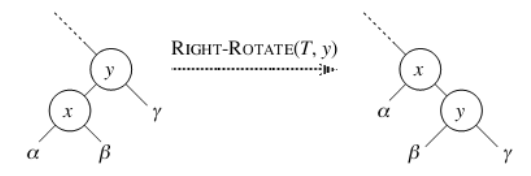
\includegraphics[scale=0.8]{p3.png}\\
This step of right rotation increases the number of nodes in the right spine by 1 and decreases the number of nodes not in the right spine by 1. Any binary search tree starts out with at least one node (the root) in the right spine. Moreover, if there are any nodes not on the right spine, then at least it has a ancestor on the right spine. Thus, at most n-1 right rotations are needed to put all nodes in the right spine, and the tree becomes a right-skewed tree.\\
If we know how to convert any arbitrary n-node binary search tree into an n-node right-skewed tree, than we know how to convert this right-skewed tree into any arbitrary n-node binary search tree. What we need to do is to reverse the sequence of the right rotation steps and change them into their inverse left rotation.\\
Therefore, we have proved that any arbitrary n-node binary search tree can be transformed into any other arbitrary n-node binary search tree using $O(n)$ rotations. 
\end{solution}

\item  Suppose that an AVL tree insertion breaks the AVL balance condition. Suppose node $P$ is the first node that has a balance condition violation in the insertion access path from the leaf. Assume the key is inserted into the left subtree of $P$ and the left child of $P$ is node $A$. Prove the following claims:
	\begin{enumerate}
		\item  Before insertion, the balance factor of node $P$ is 1. After insertion and before applying rotation to fix the violation, the balance factor of node $P$ is 2.
		\item Before insertion, the balance factor of node $A$ is 0. After insertion and before applying rotation to fix the violation, the balance factor of node $A$ cannot be 0.
	\end{enumerate}
	
\begin{solution}
\quad\\
\begin{enumerate}
\item
Suppose the balance factor of node $P$ before insertion is $x$. Correspondingly, the balance factor of node $P$ after insertion and before applying rotation to fix the violation is $x+1$ because the key is inserted into the left subtree of $P$. Since node $P$ is the first node that has a balance condition violation in the insertion access path from the leaf, we get that $x<2$ and $x+1\geq2$. Therefore, we get $x=1$. Before insertion, the balance factor of node $P$ is 1. After insertion and before applying rotation to fix the violation, the balance factor of node $P$ is 2.
\item
Before insertion, the balance factor of node $A$ has only three possible value:1,0,-1, or else it would have break the AVL balance already.
\begin{enumerate}
\item
If before insertion, the balance factor of $A$ is 1.\\
If the key is inserted into the left subtree of $A$, then the balance factor of $A$ after insertion is 2 and $A$ becomes the first node that has a balance condition violation. This contradicts with the problem statement. If the key is inserted into the right subtree of $A$, then the height of the left subtree of $P$ remains unchanged and the balance factor of $P$ remains 1 and will not break the AVL balance, which also contradicts with the problem statement. Thus, the balance factor of $A$ before insertion can't be 1.
\item
If before insertion, the balance factor of $A$ is -1.\\
If the key is inserted into the right subtree of $A$, then the balance factor of $A$ after insertion is -2 and $A$ becomes the first node that has a balance condition violation. This contradicts with the problem statement. If the key is inserted into the left subtree of $A$, then the height of the left subtree of $P$ remains unchanged and the balance factor of $P$ remains 1 and will not break the AVL balance, which also contradicts with the problem statement. Thus, the balance factor of $A$ before insertion can't be -1.
\item
Therefore, the balance factor of $A$ before insertion must be 0. Also, if we want $P$ to be the first node that violates the AVL balance, then the insertion must increase the height of the left subtree of $P$ by 1. If after one insertion, the balance factor of $A$ is still 1, then the height of $P$'s left subtree will not change. Therefore, the balance factor of node $A$ after insertion and before fixing the violation cannot be 0.
\end{enumerate}
\end{enumerate}
\end{solution}

\end{enumerate}

%========================================================================
\end{document}